
\begin{figure*}[t]
  \centering
  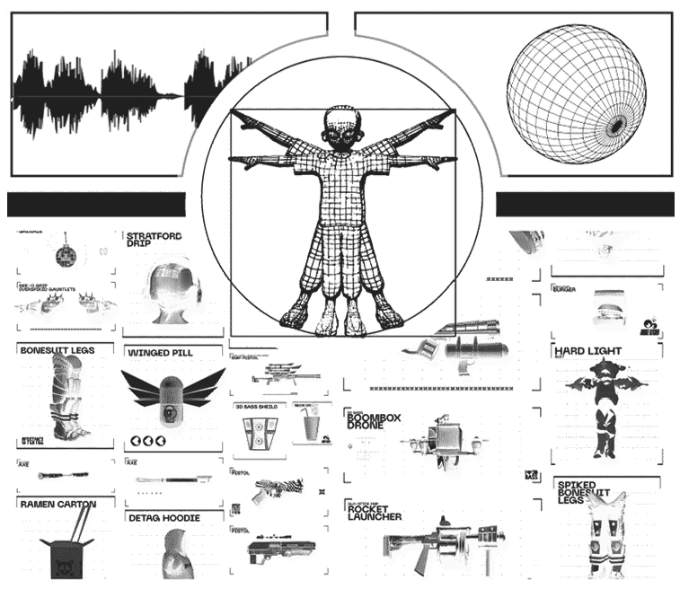
\includegraphics[width=0.9\textwidth]{images/image15.png}
  \caption{}
  \label{fig:vision}
\end{figure*}
\FloatBarrier % Prevents LaTeX from pushing content past this point
\section{Vision and Summary}

The Action substrate reimagines the digital economy for sovereign worlds, games, and communities. By combining decentralized infrastructure with creativity and shared governance, the protocol fosters originality, collaboration, and real-world impact.

\subsection{Key Highlights}
\begin{itemize}
\item \textbf{Hyperobjects}: Dynamic, interoperable assets - the connective tissue of the next Internet
\item \textbf{Action Substrate}: Decentralized compute and storage foundation
\item \textbf{ACTION Token}: Ownership, governance, and economic backbone
\item \textbf{Real World Action}: A solarpunk commitment to environmental and social good
\end{itemize}

Building on the scalable storage and compute made possible by Arweave and AO, Action aims to be a core layer of scalable gaming infrastructure for an Internet built on game engines, connected by game assets that are both interoperable and decentralized. Action sets the stage for a decentralized, collaborative metaverse built on the principles of creativity, ownership, and impact.

The Action ecosystem is designed to be a \textbf{utility-driven, decentralized framework} for self-sovereign gaming and digital asset interactions. By implementing \textbf{strong compliance measures, risk disclosures, and a structured governance transition}, Action aims to ensure \textbf{long-term sustainability and regulatory alignment}, mitigating potential legal and financial risks for participants.
